\documentclass[parskip=full]{scrartcl}
\usepackage[utf8]{inputenc} % use utf8 file encoding for TeX sources
\usepackage[T1]{fontenc}    % avoid garbled Unicode text in pdf
\usepackage[german]{babel}  % german hyphenation, quotes, etc
\usepackage{hyperref}       % detailed hyperlink/pdf configuration
\hypersetup{                % ‘texdoc hyperref‘ for options
pdftitle={Aufgabe_1},%
bookmarks=true,%
}
\usepackage{graphicx}       % provides commands for including figures
\usepackage{csquotes}       % provides \enquote{} macro for "quotes"
\usepackage[nonumberlist]{glossaries}     % provides glossary commands
\usepackage{enumitem}

\makenoidxglossaries
%
% % Glossareinträge
%
\newglossaryentry{Benutzer}
{
	name=Benutzer,
	plural=Benutzer,
	description={jemand, der etwas [leihweise] benutzt},
}

\newglossaryentry{Kunde}
{
	name=Kunde,
	plural=Kunden,
	description={(Zahlende) Teilnehmer einer oder mehrerer Seminarveranstaltung/en}
}
\newglossaryentry{Kunstfiltern}
{
	name=Kunstfilter,
	plural=Kunstfiltern,
	description={Funktion in einer Grafiksoftware, die ein bestehendes digitales Bild (meistens Rastergrafik) mit einem vorprogrammierten Algorithmus, der häufig in einigen Parametern konfigurierbar ist, gezielt verändern}
}

\newglossaryentry{Metainformationen}
{
	name=Metainformation,
	plural=Metainformationen,
	description={Information, die anderer Information übergeordnet ist}
}

\newglossaryentry{Server}
{
	name=Server,
	plural=Server,
	description={Rechner, der für andere in einem Netzwerk mit ihm verbundene Systeme bestimmte Aufgaben übernimmt und von dem diese ganz oder teilweise abhängig sind}
}

\newglossaryentry{Rechner}
{
	name=Rechner,
	description={Gerät zur Verarbeitung zur Daten, das die Daten einlesen, verarbeiten, speichern und ausgeben kann}
}

\title{iMage: Lastenheft}
\author{Kaloyan Draganov, 2313306}

\begin{document}

\maketitle

\section{Zielbestimmung}
Die Firma Pearcorp entwickelt das System iMage. iMage ist ein Bildverarbeitungssoftware Produkt mit Schwerpunkt auf \gls{Kunstfiltern}. Dem \gls{Benutzer} wird die Möglichkeit zur Verfügung gestellt, im Internet nach frei nutzbare Bilder zu suchen, sie zu bearbeiten und auf dem lokalen \gls{Rechner} oder auf dem Pearcorp \gls{Server} zu speichern.

\section{Produkteinsatz}
Das Produkt dient zur Kunden der Firma Pearcorp.

Zielgruppe: die Kunden der Firma Pearcorp.

Plattform: PC mit Windows 7 oder Nachfolger-Betriebssystem.

\section{Funktionale Anforderungen}
\begin{itemize}[nosep]
\item[FA10] Internetsuche für Bilder nach einer angegebenen Reihe von Schlüsselwörter.
\item[FA20] Internetsuche für Bilder nach einer angegebenen Reihe von Schlüsselwörter mit integrierter gleichzeitiger Komprimierung.
\item[FA30] Anzeigen von zuletzt zugegriffenen Bilder.
\item[FA40] Lokales Speichern von ausgewählten Bilder.
\item[FA50] Entferntes Speichern von ausgewählten Bilder auf einem zum System zugehörigen Zentralserver.
\end{itemize}

\section{Produktdaten}
\begin{itemize}[nosep]
\item[PD10] Es sind vom Benutzer ausgewählten Bilder zu speichern.
\item[PD20] Es sind zum Bilder gehörige \gls{Metainformationen} zu speichern. Insbesondere zählen dazu Nutzungsrechte.
\item[PD30] 
\end{itemize}

\section{Nichtfunktionale Anforderungen}
\begin{itemize}[nosep]
\item[NF10] Die Suche soll für eine Anzahl von fünfhundert (500) Bildern maximal zehn (10)Minuten benötigen und selbstständig nach einer Suchdauer von einer Stunde abbrechen.
\item[NF20] Maximal sollen 50  Bilder  gleichzeitig  angezeigt  werden.
\item[NF30] Der Zugriff auf den Zentralserver soll von mindestens einhundert (100) Nutzern gleich-zeitig erfolgen können.
\item[NF40] Die Dauer des Hochladens der Bilder maximal linear mit der Anzahl der Bilder wachsen.
\item[NF50] Der maximale Grad an Komprimierung soll dabei abhängig von der Bildgröße so berechnet werden, dass die Motive in 90\% der Bilder erkennbar bleiben.
\end{itemize}

\section{Systemmodelle}

\subsection{Szenarien}

\subsection{Anwendungsfälle}
\subsubsection{Seminarorganisation}
\begin{center}
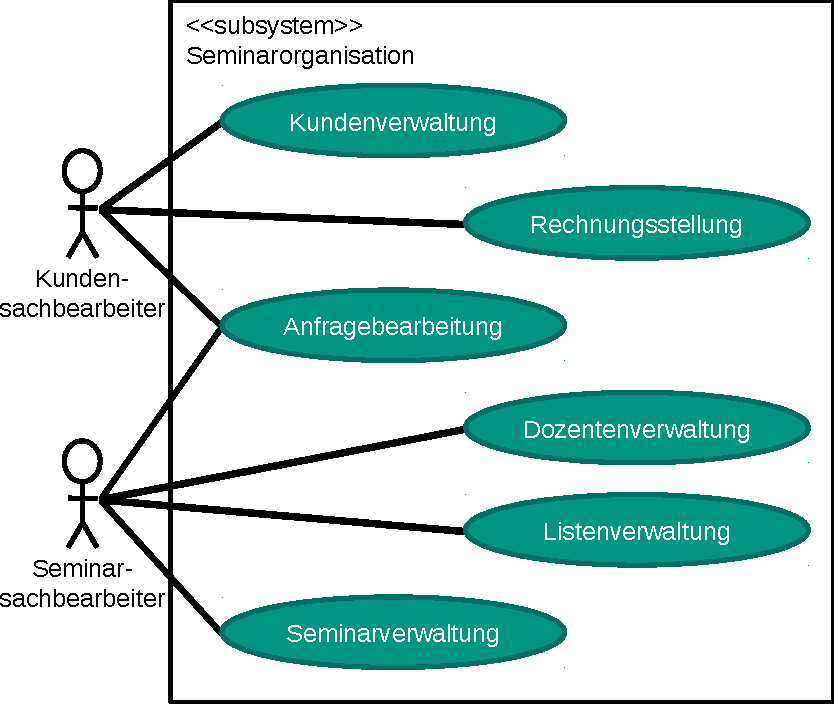
\includegraphics[width=0.8\textwidth]{szenario_seminarorganisation.pdf}
\end{center}

Akteure: Kundensachbearbeiter, Seminarsachbearbeiter.

Anwendungsfälle: Kundenverwaltung, Rechnungsstellung, Anfragebearbeitung, Dozentenverwaltung, Listenverwaltung, Seminarverwaltung.

Textuelle Beschreibung: (folgt)



%
% % Automatisch generiertes Glossar (Latex zwei mal ausführen um Glossar anzuzeigen)
%
%\glsaddall % das sorgt dafür, dass alles Glossareinträge gedruckt werden, nicht nur die verwendeten. Das sollte nicht nötig sein!
\printnoidxglossaries


\end{document}
